\everymath{\displaystyle}
\documentclass{beamer}
% \documentclass[handout]{beamer}

%\usepackage[pdftex]{color,graphicx}
\usepackage{amsmath,amssymb,amsfonts}

\mode<presentation>
{
  % \usetheme{Darmstadt}
  % \usetheme[hideothersubsections]{Hannover}
  % \usetheme[hideothersubsections]{Goettingen}
  \usetheme[hideothersubsections, right]{Berkeley}

  \usecolortheme{seahorse}
  % \usecolortheme{dolphin}
  \usecolortheme{rose}
  % \usecolortheme{orchid}

  \useinnertheme[shadow]{rounded}

  \setbeamercovered{transparent}
  % or whatever (possibly just delete it)
}

\mode<handout>{
  \setbeamercolor{background canvas}{bg=black!5}
  \usepackage{pgfpages}
  \pgfpagesuselayout{4 on 1}[a4paper,border shrink=5mm, landscape]
}

\usepackage[brazilian]{babel}
% or whatever

% \usepackage[latin1]{inputenc}
\usepackage[utf8]{inputenc}
% or whatever

\usepackage{times}
%\usepackage[T1]{fontenc}
% Or whatever. Note that the encoding and the font should match. If T1
% does not look nice, try deleting the line with the fontenc.


\title%[] % (optional, use only with long paper titles)
{Tópicos em resultados preliminares}

\subtitle
{Análise Exploratória de Dados} % (optional)

\author%[] % (optional, use only with lots of authors)
{Felipe Figueiredo}% \and S.~Another\inst{2}}
% - Use the \inst{?} command only if the authors have different
%   affiliation.

\institute[INTO] % (optional, but mostly needed)
{Instituto Nacional de Traumatologia e Ortopedia
}
  % \inst{1}%
  % Department of Computer Science\\
  % University of Somewhere
  % \and
  % \inst{2}%
  % Department of Theoretical Philosophy\\
  % University of Elsewhere}
% - Use the \inst command only if there are several affiliations.
% - Keep it simple, no one is interested in your street address.

\date%[] % (optional)
{}

% \subject{Talks}
% This is only inserted into the PDF information catalog. Can be left
% out. 



% If you have a file called "university-logo-filename.xxx", where xxx
% is a graphic format that can be processed by latex or pdflatex,
% resp., then you can add a logo as follows:

\pgfdeclareimage[height=1.6cm]{university-logo}{../logo}
\logo{\pgfuseimage{university-logo}}



% Delete this, if you do not want the table of contents to pop up at
% the beginning of each subsection:
\AtBeginSubsection[]
%\AtBeginSection[]
{
  \begin{frame}<beamer>{Sumário}
    \tableofcontents[currentsection,currentsubsection]
  \end{frame}
}


% If you wish to uncover everything in a step-wise fashion, uncomment
% the following command: 

% \beamerdefaultoverlayspecification{<+->}


\begin{document}

\begin{frame}
  \titlepage
\end{frame}

\begin{frame}{Sumário}
  \tableofcontents
  % You might wish to add the option [pausesections]
\end{frame}


%% Template
% \section{}

% \subsection{}

% \begin{frame}{}
%   \begin{itemize}
%   \item 
%   \end{itemize}
% \end{frame}

% \begin{frame}
%   \begin{columns}
%     \begin{column}{5cm}
%     \end{column}
%     \begin{column}{5cm}
%     \end{column}
%   \end{columns}
% \end{frame}

% \begin{frame}{}
%   \includegraphics[height=0.4\textheight]{file1}
%   \includegraphics[height=0.4\textheight]{file2}
%   \includegraphics[height=0.4\textheight]{file3}
%   \begin{figure}
%     \caption{}
%   \end{figure}
% \end{frame}

% \begin{frame}{}
%   \begin{definition}
%   \end{definition}
%   \begin{example}
%   \end{example}
%   \begin{block}{Exercício}
%   \end{block}
% \end{frame}

% \section{Discussão da aula passada}

% \subsection{Discussão da aula passada}

\begin{frame}{Discussão da aula passada}
  \begin{block}{}
    Discussão da leitura obrigatória da aula passada
  \end{block}
\end{frame}

\section{Análise Exploratória}

\subsection{EDA}

\begin{frame}
  \begin{block}{Evidências}
    \footnotesize
    ``{\em
      It is a capital mistake to theorize before one has data.
      Insensibly one begins to twist facts to suit theories, instead
      of theories to suit facts.}''

  \bigskip
  \hfill \tiny Sherlock Holmes
  \end{block}
\end{frame}

\begin{frame}{Paradigmas de Análises de Dados}
  \footnotesize
  Estudos quantitativos requerem coleta e análise de dados
  \bigskip
  \bigskip
  \begin{itemize}
  \item \alert<2>{EDA -- Análise Exploratória de Dados}
  \bigskip
  \item CDA -- Análise Confirmatória de Dados
  \end{itemize}
\end{frame}

\begin{frame}{Análise Exploratória de Dados}
  \begin{itemize}
    \footnotesize
  \item<1-> Formalizado por John W. Tukey nos anos 1970
  \bigskip
  \item<1-> Objetivo: formular perguntas com base nos dados disponíveis
  \bigskip
  \item<2-> Perguntas que podem ser respondidas pela análise dos dados
  \end{itemize}
\end{frame}

\begin{frame}{Análise Exploratória de Dados}
  \begin{block}{O que é}
    \scriptsize
    Uma filosofia/approach para

    \bigskip
    \begin{itemize}
      \footnotesize
    \item insight sobre um dataset
      \medskip
    \item descobrir estruturas/padrões
      \medskip
    \item identificar variáveis importantes
      \medskip
    \item detectar outliers e anomalias
    \end{itemize}
  \end{block}

  \vfill
  \scriptsize
  \hfill \href{https://www.itl.nist.gov/div898/handbook/eda/section1/eda16.htm}
  {NIST Handbook (1998)}
\end{frame}

\begin{frame}{Análise Exploratória de Dados}
  \begin{block}{Do resumo...}
    \footnotesize {\em ``Ideas come from previous exploration more
      often than from lightning strokes. Important questions can
      demand the most careful planning for confirmatory
      analysis. (\ldots) \alert<2>{Finding the question is often more
        important than finding the answer.} Exploratory data analysis
      is an atitude, (\ldots) NOT a bundle of techniques (\ldots).''}
  \end{block}

  \vfill
  \scriptsize
  \hfill Tukey, 1980
\end{frame}

% \begin{frame}{Análise Exploratória de Dados}
%   \begin{block}{Para Tukey:}
%     \begin{itemize}
%       \footnotesize
%     \item Não basta fazer a análise confirmatória, nem a exploratória:
%       \alert{ambas} são necessárias
%       \bigskip
%     \item Paradigma: pergunta $\rightarrow$ resposta é inadequado
%       \bigskip
%     \item ``Encontrar a pergunta é por vezes mais importante que
%       encontrar a resposta''
%     \end{itemize}
%   \end{block}

%   \vfill
%   \tiny
%   \hfill Tukey, 1980
% \end{frame}

\begin{frame}{Mapa}
  \begin{enumerate}
    \scriptsize
  \item Um paradigma incompleto
    \bigskip
  \item Origem das ideias
    \bigskip
  \item Perguntas importantes
    \bigskip
  \item A investigação abrangente
    \bigskip
  \item Uma máxima
    \bigskip
  \item Análise confirmatória
  \end{enumerate}

  \vfill
  \scriptsize
  \hfill Tukey, 1980
\end{frame}

\begin{frame}{Paradigma linear -- incompleto}
  \begin{center}
    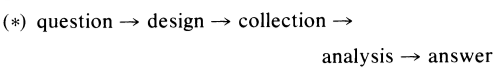
\includegraphics[width=0.7\textwidth]{EDA/eda-tukey1}
  \end{center}
  \bigskip
  \begin{block}{\scriptsize Este paradigma simplista presume que...}
    \begin{itemize}
      \footnotesize
    \item Sabemos a pergunta ``correta'' no início
      \bigskip
    \item Ignora questões importantes sobre o processo investigativo
      \medskip
      \begin{itemize}
        \tiny
      \item<2> Como as perguntas são geradas?
        \medskip
      \item<2> Como os desenhos (experimentais) são guiados?
        \medskip
      \item<2> Como a coleta de dados é monitorada?
      \end{itemize}
    \end{itemize}
  \end{block}

  \vfill
  \scriptsize
  \hfill Tukey, 1980
\end{frame}

\begin{frame}{Paradigma linear -- incompleto}
  \begin{center}
    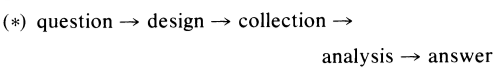
\includegraphics[width=0.7\textwidth]{EDA/eda-tukey1}
  \end{center}
  \bigskip
  \begin{block}{Como as perguntas são geradas?}
    \footnotesize
    Geralmente por {\em insights} teóricos e a exploração de dados anteriores (e.g., pesquisa bibliográfica)
  \end{block}

  \vfill
  \scriptsize
  \hfill Tukey, 1980
\end{frame}

\begin{frame}{Paradigma linear -- incompleto}
  \begin{center}
    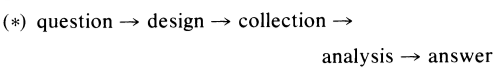
\includegraphics[width=0.7\textwidth]{EDA/eda-tukey1}
  \end{center}
  \bigskip
  \begin{block}{Como os desenhos (experimentais) são guiados?}
    \footnotesize
    Geralmente por informação qualitativa disponível
    obtida da exploração de dados anteriores
\end{block}

  \vfill
  \scriptsize
  \hfill Tukey, 1980
\end{frame}

\begin{frame}{Paradigma linear -- incompleto}
  \begin{center}
    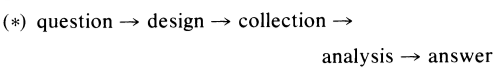
\includegraphics[width=0.7\textwidth]{EDA/eda-tukey1}
  \end{center}
  \bigskip
  \begin{block}{Como a coleta de dados é monitorada?}
    \footnotesize
    Geralmente pela exploração dos dados, conforme são obtidos, buscando
    comportamento ``inesperado''
  \end{block}

  \vfill
  \scriptsize
  \hfill Tukey, 1980
\end{frame}

\begin{frame}{Explorar\ldots}
  \begin{itemize}
    \footnotesize
  \item A chave então é explorar os dados
    \bigskip
  \item Explorar antes, durante e depois da análise confirmatória
    \bigskip
  \item Busca de pistas, ideias e eventualmente conclusões
    preliminares ({\em hipóteses}!)
  \end{itemize}

  \vfill
  \scriptsize
  \hfill Tukey, 1980
\end{frame}

\begin{frame}{A origem das ideias}
  \begin{center}
    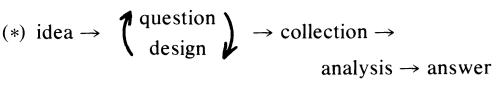
\includegraphics[width=0.7\textwidth]{EDA/eda-tukey2}
  \end{center}
  \scriptsize
  Tukey sugere que:
  \bigskip
  \begin{itemize}
    \footnotesize
  \item Antes de termos uma pergunta, temos uma ideia (a ser
    formalizada)\footnote{\scriptsize Assim como sua ``proposta de pergunta 1/2''}
    \bigskip
  \item Pergunta formal depende dos dados disponíveis
    \bigskip
  \item Questão pragmática, independe do desejo ou vontade
  \end{itemize}

  \vfill
  \scriptsize
  \hfill Tukey, 1980
\end{frame}

\begin{frame}{A origem das ideias}
  \begin{exampleblock}{Exemplo}
    \begin{itemize}
      \scriptsize
    \item<1-> Ideia: uma certa droga ajuda em uma doença
    \item<2-> Queremos testar/confirmar isso\ldots
    \item<3-> \ldots com consistência estatística na resposta
    \end{itemize}
  \end{exampleblock}
  \bigskip
  \begin{itemize}
  \item<1-> Ideia preliminar informal, vaga
    \bigskip
  \item<1-> Geralmente em termos de linguagem coloquial
    \bigskip
  \item<3-> Não pode ser avaliada com suporte estatístico
  \end{itemize}

  \vfill
  \scriptsize
  \hfill Tukey, 1980
\end{frame}

\begin{frame}{A origem das ideias}
  \scriptsize
  Desejo: pergunta geral, de amplo espectro e implicações profundas
  \bigskip
  \begin{exampleblock}{Exemplo}
    \scriptsize
    ``Dos pacientes que morreriam em até três anos desta doença, que
    proporção poderia ser salva por este tratamento?''
  \end{exampleblock}
  \bigskip
  \begin{itemize}
    \footnotesize
  \item Dificuldade técnica\footnote{Neste exemplo, questão ética}\ldots
    \bigskip
  \item \ldots nenhum design pode isolar essas pessoas para um experimento
  \end{itemize}

  \vfill
  \scriptsize
  \hfill Tukey, 1980
\end{frame}

\begin{frame}{A origem das ideias}
  \scriptsize
  O que \alert{pode} ser perguntado está limitado por:
  \bigskip
  \begin{itemize}
    \footnotesize
  \item Idade e sexo dos pacientes
    \bigskip
  \item conjunto mínimo de sintomas
    \bigskip
  \item ausência de outras condições potencialmente fatais
    \bigskip
  \item tipos de pacientes que podem ser encontrados/observados
    \bigskip
  \item etc.
  \end{itemize}

  \vfill
  \scriptsize
  \hfill Tukey, 1980
\end{frame}

\begin{frame}{A origem das ideias}
  \begin{itemize}
    \footnotesize
  \item o que pode concretamente ser perguntado
    \bigskip
  \item que desenhos são viáveis
    \bigskip
  \item chance de um certo design resultar em resposta útil
  \end{itemize}
  \bigskip
  \begin{block}{}
    { ``Como eu estudo o que está acontecendo aqui?''}
  \end{block}

  \vfill
  \scriptsize
  \hfill Tukey, 1980
\end{frame}

\begin{frame}{Por onde começar?}
  \begin{itemize}
    \footnotesize
  \item tabelas
    \bigskip
  \item gráficos dos dados brutos
    \bigskip
  \item estatísticas descritivas simples
    \bigskip
  \item procurar padrões
  \end{itemize}
\end{frame}

\subsection{Tabelas}

\begin{frame}
  \begin{exampleblock}{Exemplo}
    \begin{center}
      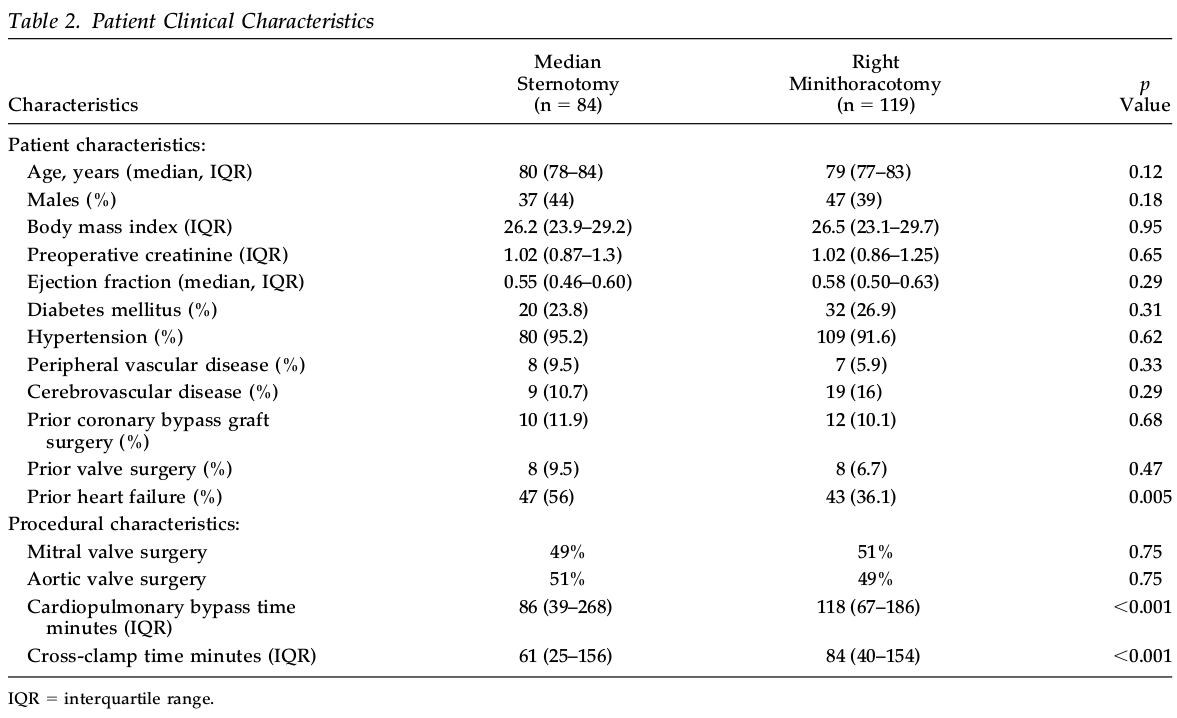
\includegraphics[width=.9\textwidth]{EDA/eda-tabela}
    \end{center}
  \end{exampleblock}

  \vfill
  \tiny
  \hfill \href{https://doi.org/10.1016/j.athoracsur.2010.09.019}{Lamelas, et al; 2011}
\end{frame}

\begin{frame}{Tabelas}
  \begin{exampleblock}{Exemplo}
    \scriptsize
    Pacientes que tem uma enfermidade grave, podem ser submetidos a um tratamento cirúrgico.

    \bigskip
    \begin{center}
    \begin{tabular}{l|cc|c}
      &Óbito & não óbito & Total\\
      \hline
      Cirurgia & 3 & 1 & 4 \\
      não cirurgia & 2 & 5 & 7\\
      \hline
      Total & 5 & 6 & 11
    \end{tabular}
    \end{center}
  \end{exampleblock}

  \bigskip
  \begin{block}{Exercício}
    % \footnotesize
    Formule uma pergunta sobre este contexto.
  \end{block}
\end{frame}

% \begin{frame}{Tabelas 2}
%   \begin{example}
%     Pacientes que tem uma efermidade grave, podem ser submetidos a um tratamento cirúrgico.

% \bigskip

%     \begin{tabular}{l|cc|c}
%       &Óbito & não óbito & Total\\
%       \hline
%       Cirurgia & 15 & 5 & 20 \\
%       não cirurgia & 10 & 24 & 34\\
%       \hline
%       Total &  & 6 & 
%     \end{tabular}
%   \end{example}
% % \uncover{  \begin{example}
% %     Este tratamento reduz a mortalidade?
% %   \end{example}
% % }
% \end{frame}

\subsection{Figuras}

% \subsubsection{Histogramas}

\begin{frame}{Histograma}
  \begin{itemize}
    \footnotesize
  \item Gráfico de barras com frequências dos dados
    \bigskip
  \item visualização prática da distribuição dos dados
    \bigskip
  \item identificar simetria, tendência central, dispersão, etc
  \end{itemize}
\end{frame}

\begin{frame}
  \begin{exampleblock}{Exemplo}
    \begin{center}
      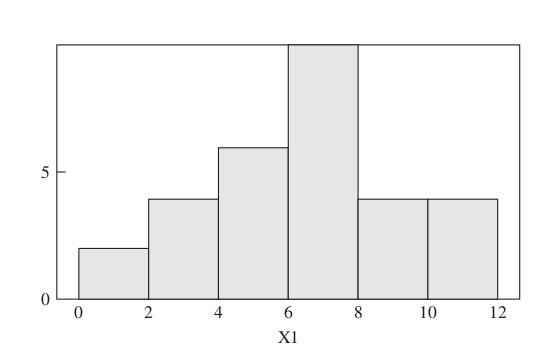
\includegraphics[height=0.7\textheight]{EDA/eda-histograma1}
    \end{center}
  \end{exampleblock}

  \vfill
  \scriptsize
  \hfill \href{https://doi.org/10.1002/0471264385.wei0202}
  {Behrens, Yu (2003)}
\end{frame}

\begin{frame}
  \begin{columns}
    \begin{column}{.5\textwidth}
      \begin{itemize}
        \tiny
      \item<2> Mensurações mais frequentes no centro
      \item<3,4> Mensurações altas/baixas menos frequentes...
      \item<4> ... com frequências semelhantes (simetria)
      \item<5> Ideia da variabilidade das mensurações (``largura'')
      \end{itemize}
    \end{column}
    \begin{column}{.5\textwidth}
      \begin{center}
        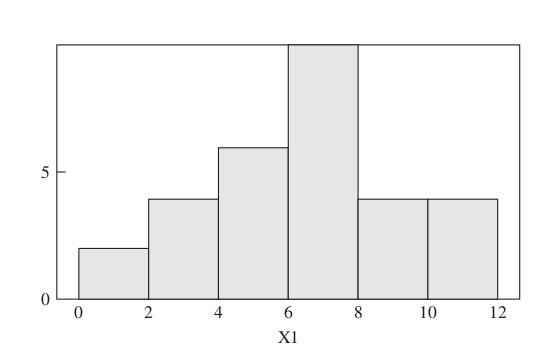
\includegraphics[width=1.35\textwidth]{EDA/eda-histograma1}
      \end{center}
    \end{column}
  \end{columns}
\end{frame}

\begin{frame}
  \begin{exampleblock}{\scriptsize Distribuições de dados podem ter várias formas}
    \begin{center}
      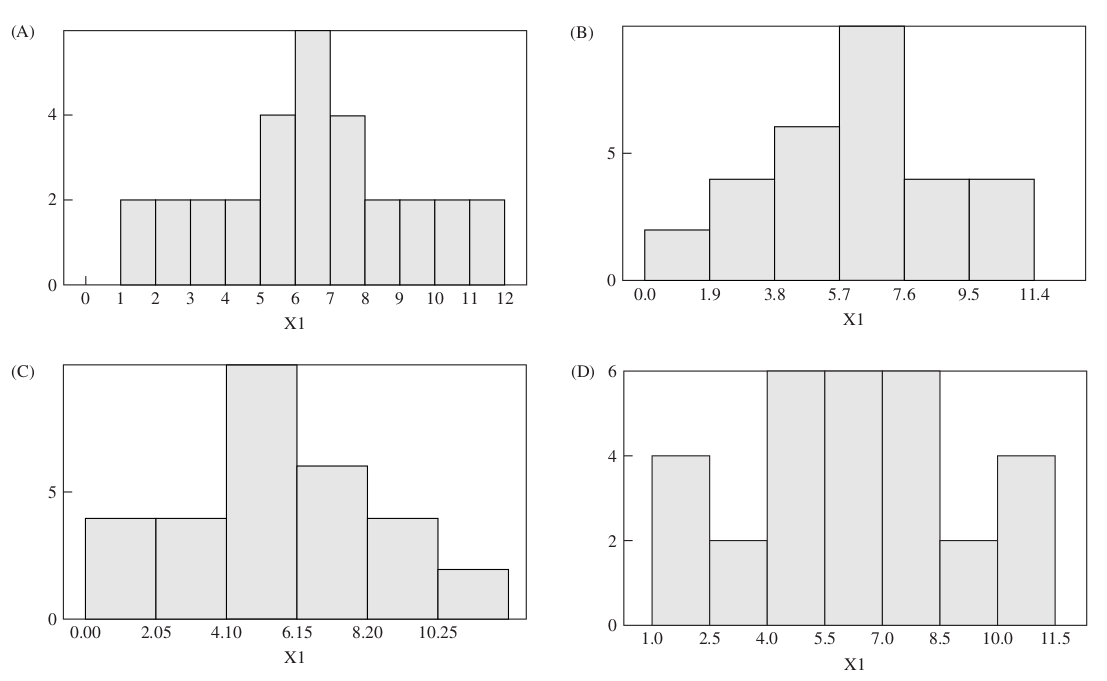
\includegraphics[width=1\textwidth]{EDA/eda-histograma2}
    \end{center}
  \end{exampleblock}
\end{frame}

% \subsubsection{Boxplot}

\begin{frame}{Boxplot}
  \begin{itemize}
    \footnotesize
  \item Mensurações feitas em dois ou mais grupos\footnote{\tiny e.g., exposição/tratamento 1, tratamento 2, controle...}
    \bigskip
  \item caixa que contém 50\% dos dados\ldots
  \item \ldots e segmentos verticais que englobam a maior parte dos
    dados
    \bigskip
  \item mensurações fora dos limites $\Rightarrow$ investigar
    possíveis outliers\footnote{\tiny erros de mensuração, imputação, viés de seleção/amostragem, observações raras...?}
    \bigskip
  \item Ideal para grandes quantidades de dados
  \end{itemize}
\end{frame}

\begin{frame}{Dotplot}
  \begin{exampleblock}{Exemplo}
    \begin{center}
      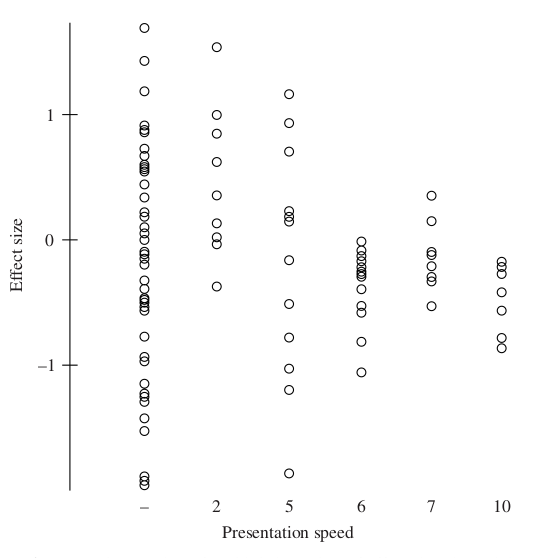
\includegraphics[height=0.7\textheight]{EDA/eda-boxplot1}
    \end{center}
  \end{exampleblock}

  \vfill
  \scriptsize
  \hfill \href{https://doi.org/10.1002/0471264385.wei0202}
  {Behrens, Yu (2003)}
\end{frame}

\begin{frame}{Boxplot}
  \begin{exampleblock}{Exemplo}
    \begin{center}
      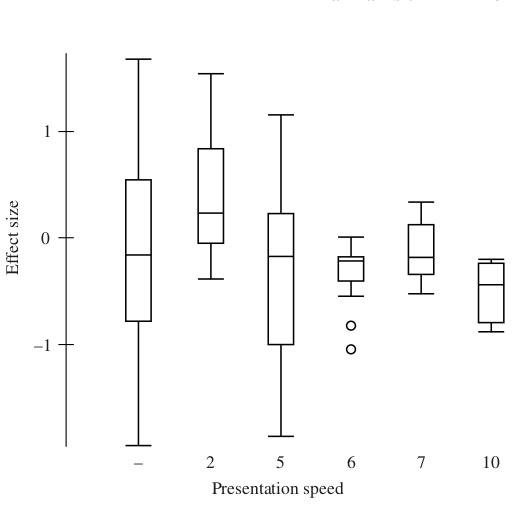
\includegraphics[height=0.7\textheight]{EDA/eda-boxplot2}
    \end{center}
  \end{exampleblock}

  \vfill
  \scriptsize
  \hfill \href{https://doi.org/10.1002/0471264385.wei0202}
  {Behrens, Yu (2003)}
\end{frame}

\begin{frame}
  \begin{columns}
    \begin{column}{.5\textwidth}
      \begin{center}
        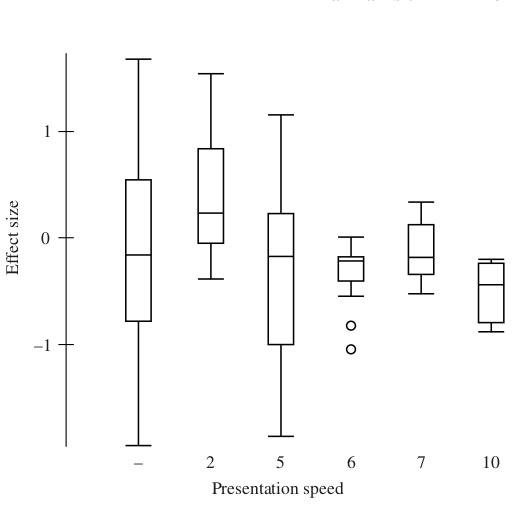
\includegraphics[width=\textwidth]{EDA/eda-boxplot2}
      \end{center}
    \end{column}
    \begin{column}{.5\textwidth}
      \begin{center}
        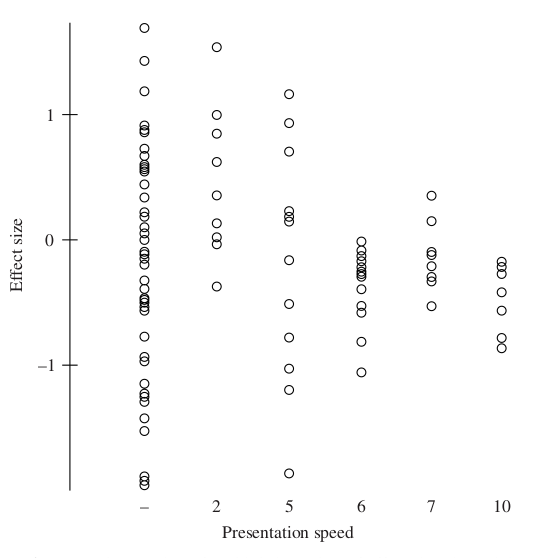
\includegraphics[width=\textwidth]{EDA/eda-boxplot1}
      \end{center}
    \end{column}
  \end{columns}
\end{frame}

% \subsubsection{Gráfico de Dispersão}

\begin{frame}{Gráficos de dispersão}
  % \scriptsize
  % Gráficos de dispersão (ou scatter-plots):
  % \bigskip
  \begin{itemize}
    \footnotesize
  \item visualizar os dados pontuais diretamente
    \bigskip
  \item identificar possíveis padrões ou tendências
    \bigskip
  \item identificar visualmente possíveis outliers
    \bigskip
  \item desenhar possíveis relações (modelos) sobre os dados
  \end{itemize}
\end{frame}

\begin{frame}
  \begin{block}{}
    \begin{center}
      A álgebra mente...

      \bigskip
      ... portanto figuras são necessárias
    \end{center}
  \end{block}

  \vfill
  \tiny
  \hfill \href{https://doi.org/10.1002/0471264385.wei0202}
  {Behrens, Yu (2003)}
\end{frame}

\begin{frame}
  \begin{exampleblock}{\scriptsize Datasets didáticos de Anscombe, 1973}
    \begin{center}
      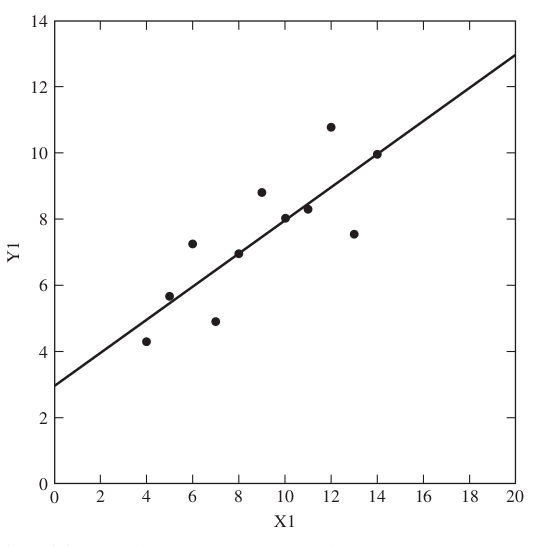
\includegraphics[width=.25\textwidth]{EDA/eda-dispersao1}
      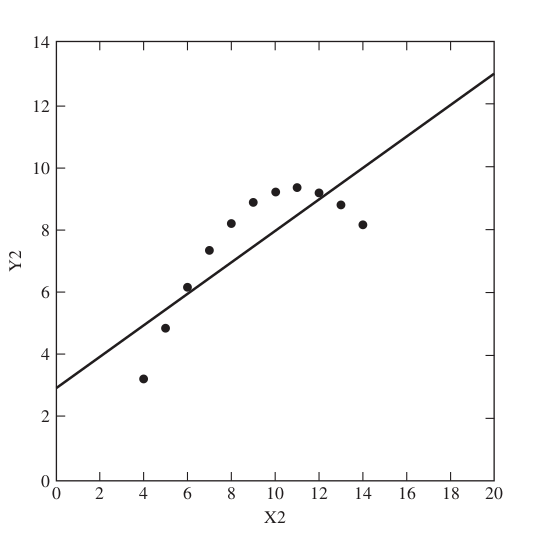
\includegraphics[width=.25\textwidth]{EDA/eda-dispersao2}

      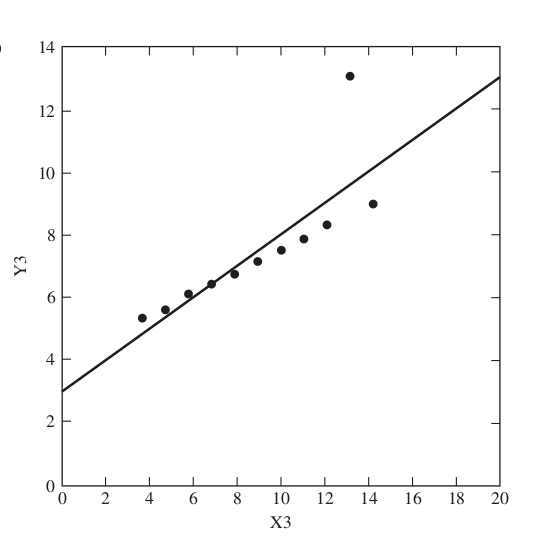
\includegraphics[width=.25\textwidth]{EDA/eda-dispersao3}
      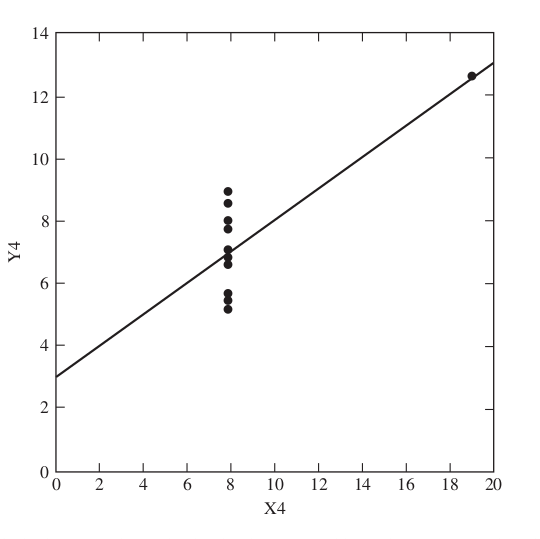
\includegraphics[width=.25\textwidth]{EDA/eda-dispersao4}
    \end{center}
  \end{exampleblock}

  \vfill
  \tiny
  Quatro datasets com perfis

  completamente diferentes $\Rightarrow$ mesma reta de melhor ajuste

  \hfill \href{https://doi.org/10.1002/0471264385.wei0202}
  {Behrens, Yu (2003)}

  \hfill \href{https://www.itl.nist.gov/div898/handbook/eda/section1/eda16.htm}
  {NIST Handbook (1998)}
\end{frame}

\begin{frame}{}
  \begin{columns}
    \begin{column}{.5\textwidth}
      \begin{itemize}
        \tiny
      \item<2-4> Relação ``claramente'' linear...
      \item<2-4> ... alguma dispersão
        \begin{itemize}
          \tiny
        \item<4> Não há justificativa para um modelo mais
          complexo (quadrático, etc...)
      \end{itemize}
      \item<5> Não há outliers
      \item<6,7> Distância vertical à reta (Y) semelhante ao longo da faixa (X)
        \begin{itemize}
          \tiny
        \item<7> Não é necessário aplicar ponderações ou transformações
        \end{itemize}
      \end{itemize}
    \end{column}
    \begin{column}{.5\textwidth}
      \begin{center}
        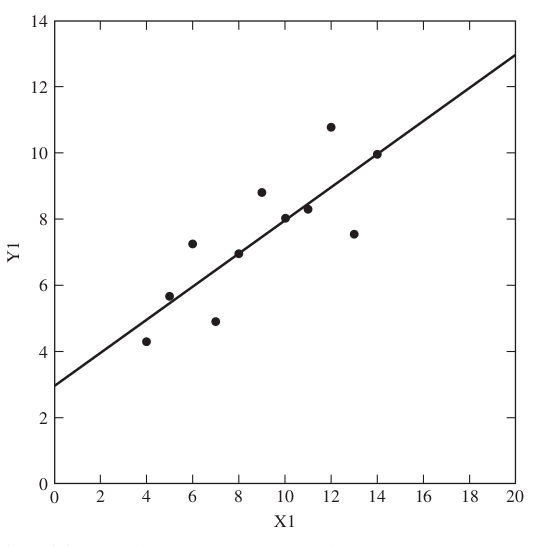
\includegraphics[width=\textwidth]{EDA/eda-dispersao1}
      \end{center}
    \end{column}
  \end{columns}
\end{frame}

\begin{frame}
  \begin{columns}
    \begin{column}{.5\textwidth}
      \begin{itemize}
        \tiny
      \item<2> Relação claramente não é linear
      \item<3> Relação ``claramente'' quadrática
      \end{itemize}
    \end{column}
    \begin{column}{.5\textwidth}
      \begin{center}
        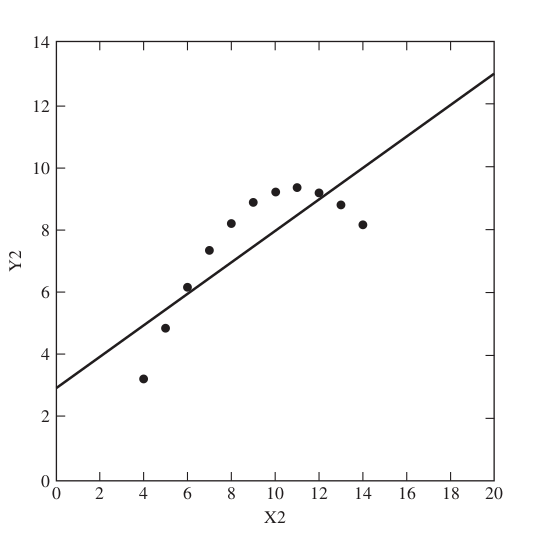
\includegraphics[width=\textwidth]{EDA/eda-dispersao2}
      \end{center}
    \end{column}
  \end{columns}
\end{frame}

\begin{frame}
  \begin{columns}
    \begin{column}{.5\textwidth}
      \begin{itemize}
        \tiny
      \item<2> ``Claramente'' possui um outlier
      \item<3> ... que ``puxa'' a reta para cima
      \end{itemize}
    \end{column}
    \begin{column}{.5\textwidth}
      \begin{center}
        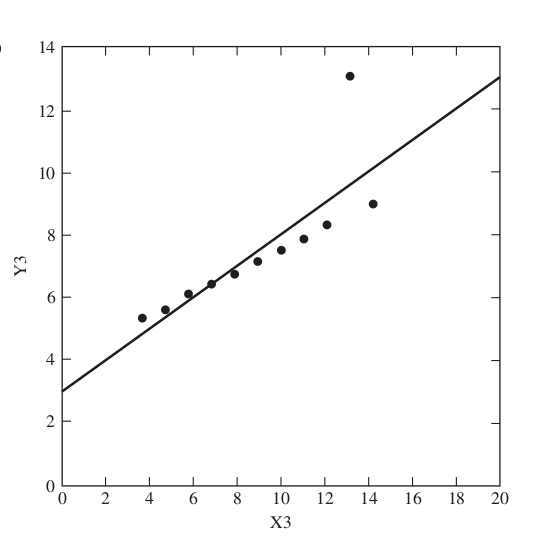
\includegraphics[width=\textwidth]{EDA/eda-dispersao3}
      \end{center}
    \end{column}
  \end{columns}
\end{frame}

\begin{frame}
  \begin{columns}
    \begin{column}{.5\textwidth}
      \begin{itemize}
        \tiny
      \item<2> CLARAMENTE vítima de um desenho experimental infeliz\footnote{Não assistiu a aula de Planejamento/Protocolo}
      \item<3,4> Um único ponto afastado do cluster de dados
      \item<4> ``cauda abanando o cachorro''
      \end{itemize}
    \end{column}
    \begin{column}{.5\textwidth}
      \begin{center}
        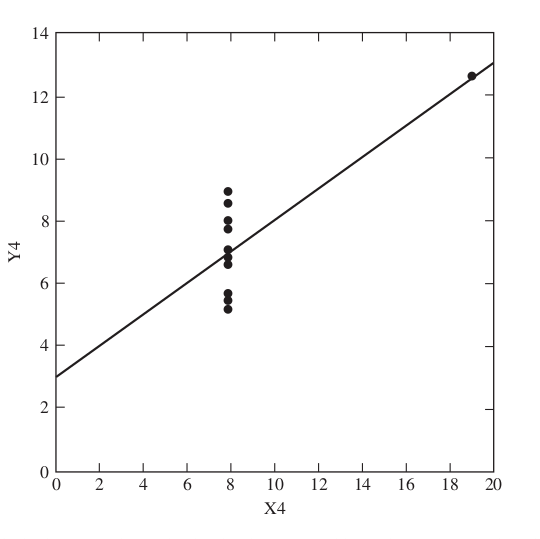
\includegraphics[width=\textwidth]{EDA/eda-dispersao4}
      \end{center}
    \end{column}
  \end{columns}
\end{frame}

\subsection{Exercício}

\begin{frame}
  \begin{center}
    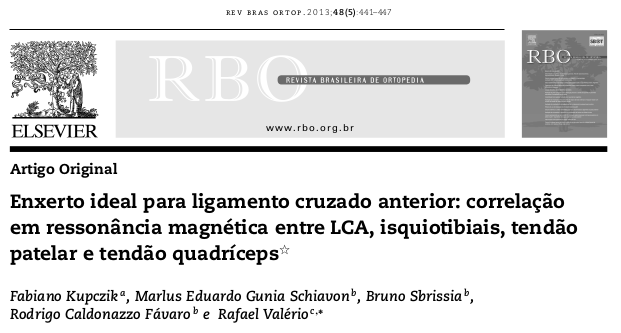
\includegraphics[width=\textwidth]{EDA/eda-exercicio1}
  \end{center}
\end{frame}

\begin{frame}
  \begin{center}
    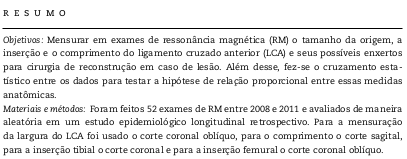
\includegraphics[width=\textwidth]{EDA/eda-exercicio2}
  \end{center}
\end{frame}

\begin{frame}
  \begin{center}
    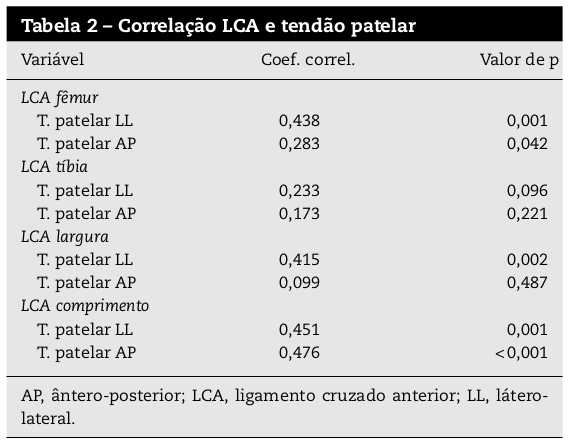
\includegraphics[height=.9\textheight]{EDA/eda-exercicio3}
  \end{center}
\end{frame}

\begin{frame}{\scriptsize Que pergunta este gráfico lhe motiva?}
  \begin{center}
    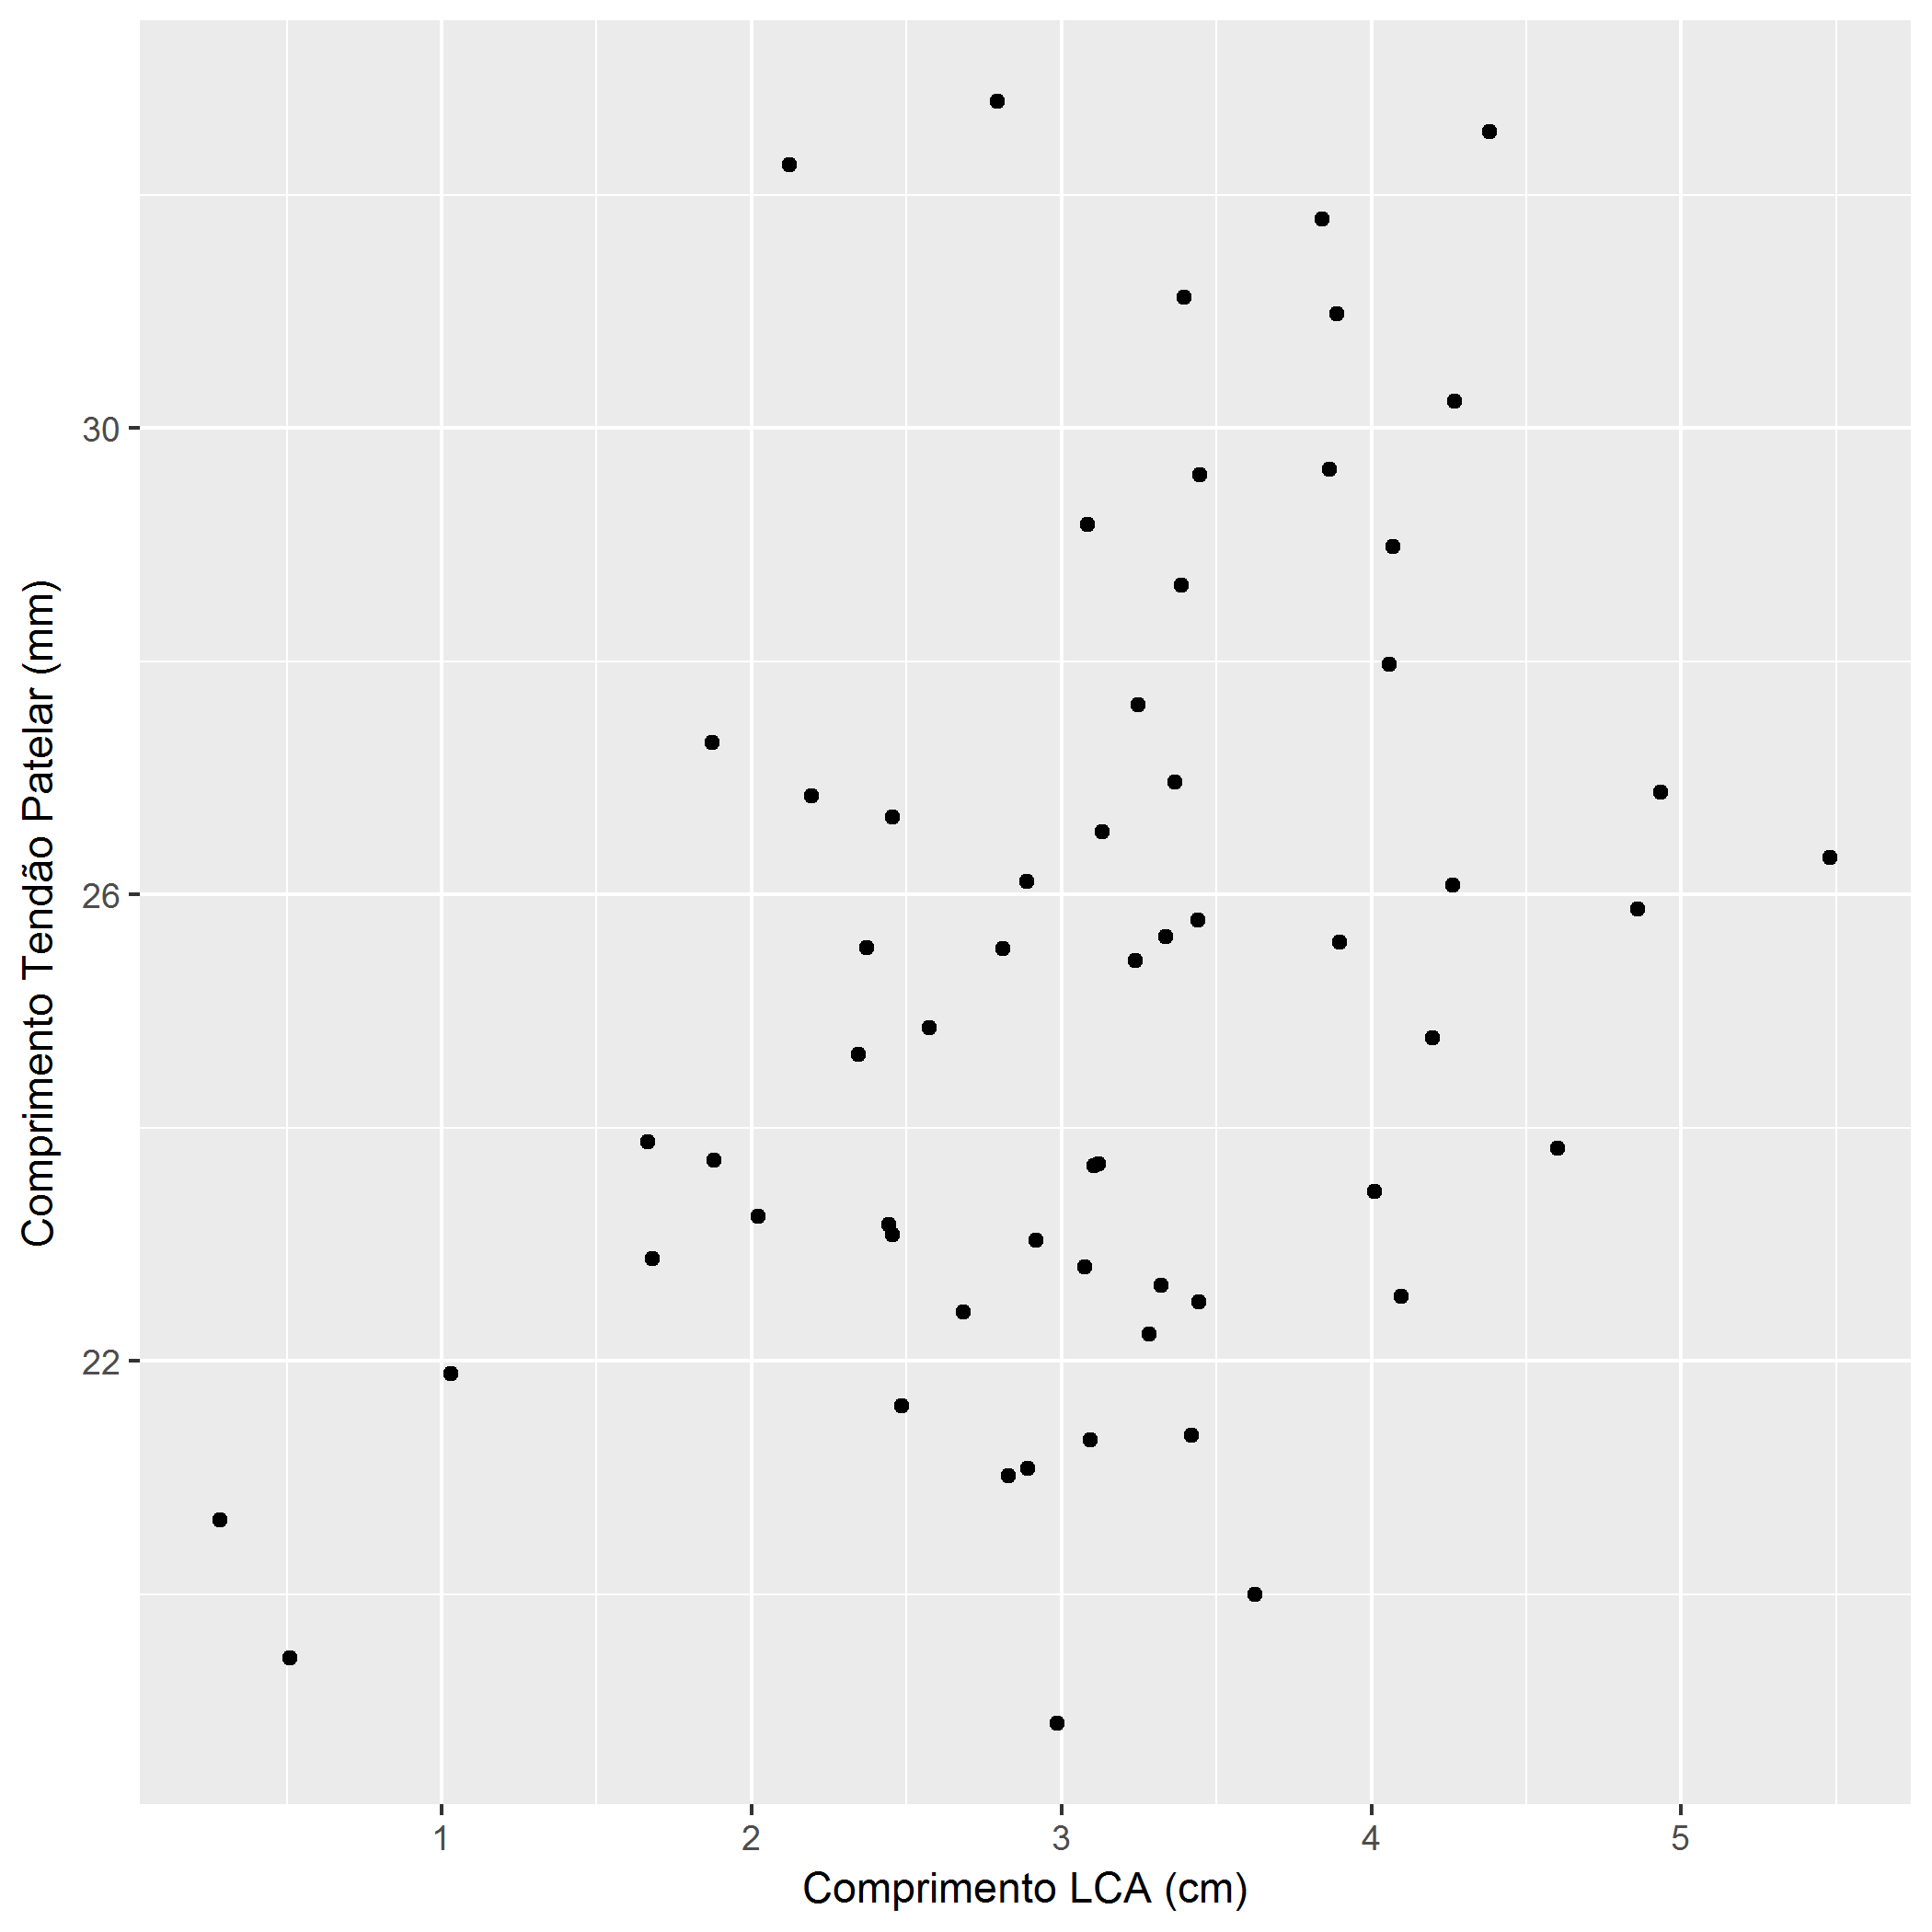
\includegraphics[height=.8\textheight]{EDA/EDA-corr1}
  \end{center}

  \vfill
  \tiny
  \hfill dados simulados com base no artigo
\end{frame}

\begin{frame}{\scriptsize O Gênero parece influenciar?}
  \begin{center}
    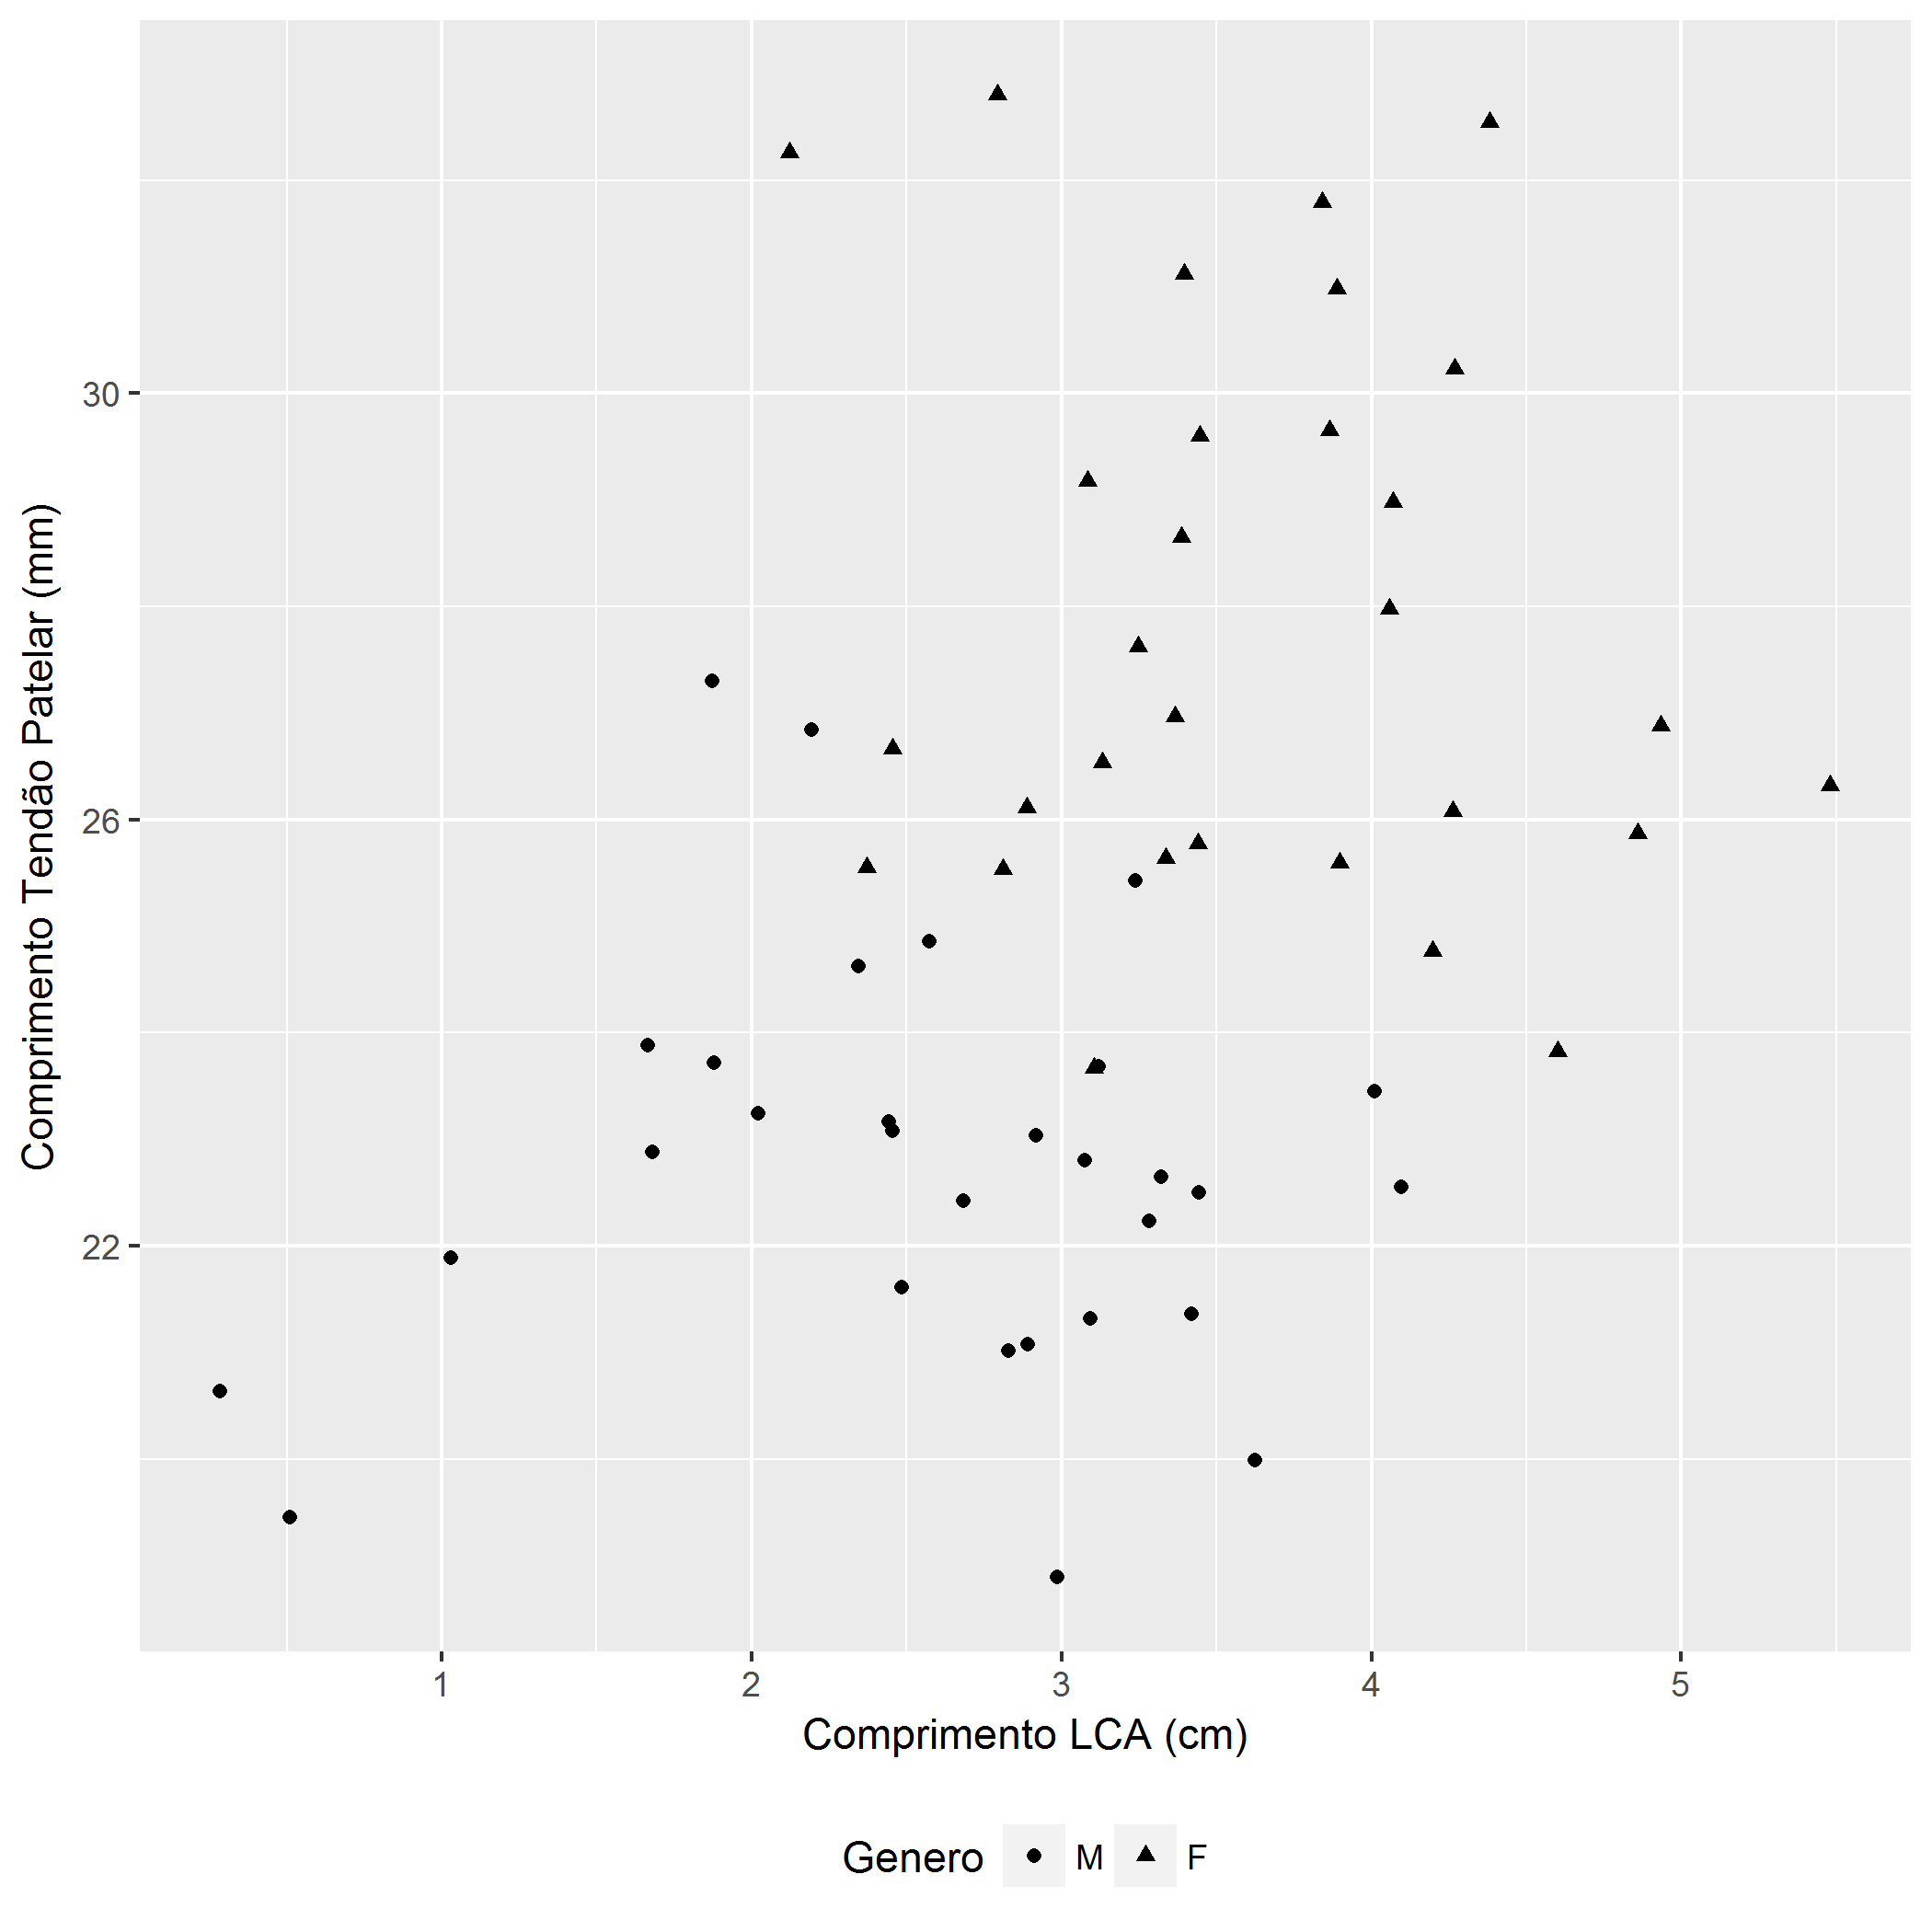
\includegraphics[height=.8\textheight]{EDA/EDA-corr2}
  \end{center}

  \vfill
  \tiny
  \hfill dados simulados com base no artigo
\end{frame}

\begin{frame}{\scriptsize E a idade?}
  \begin{center}
    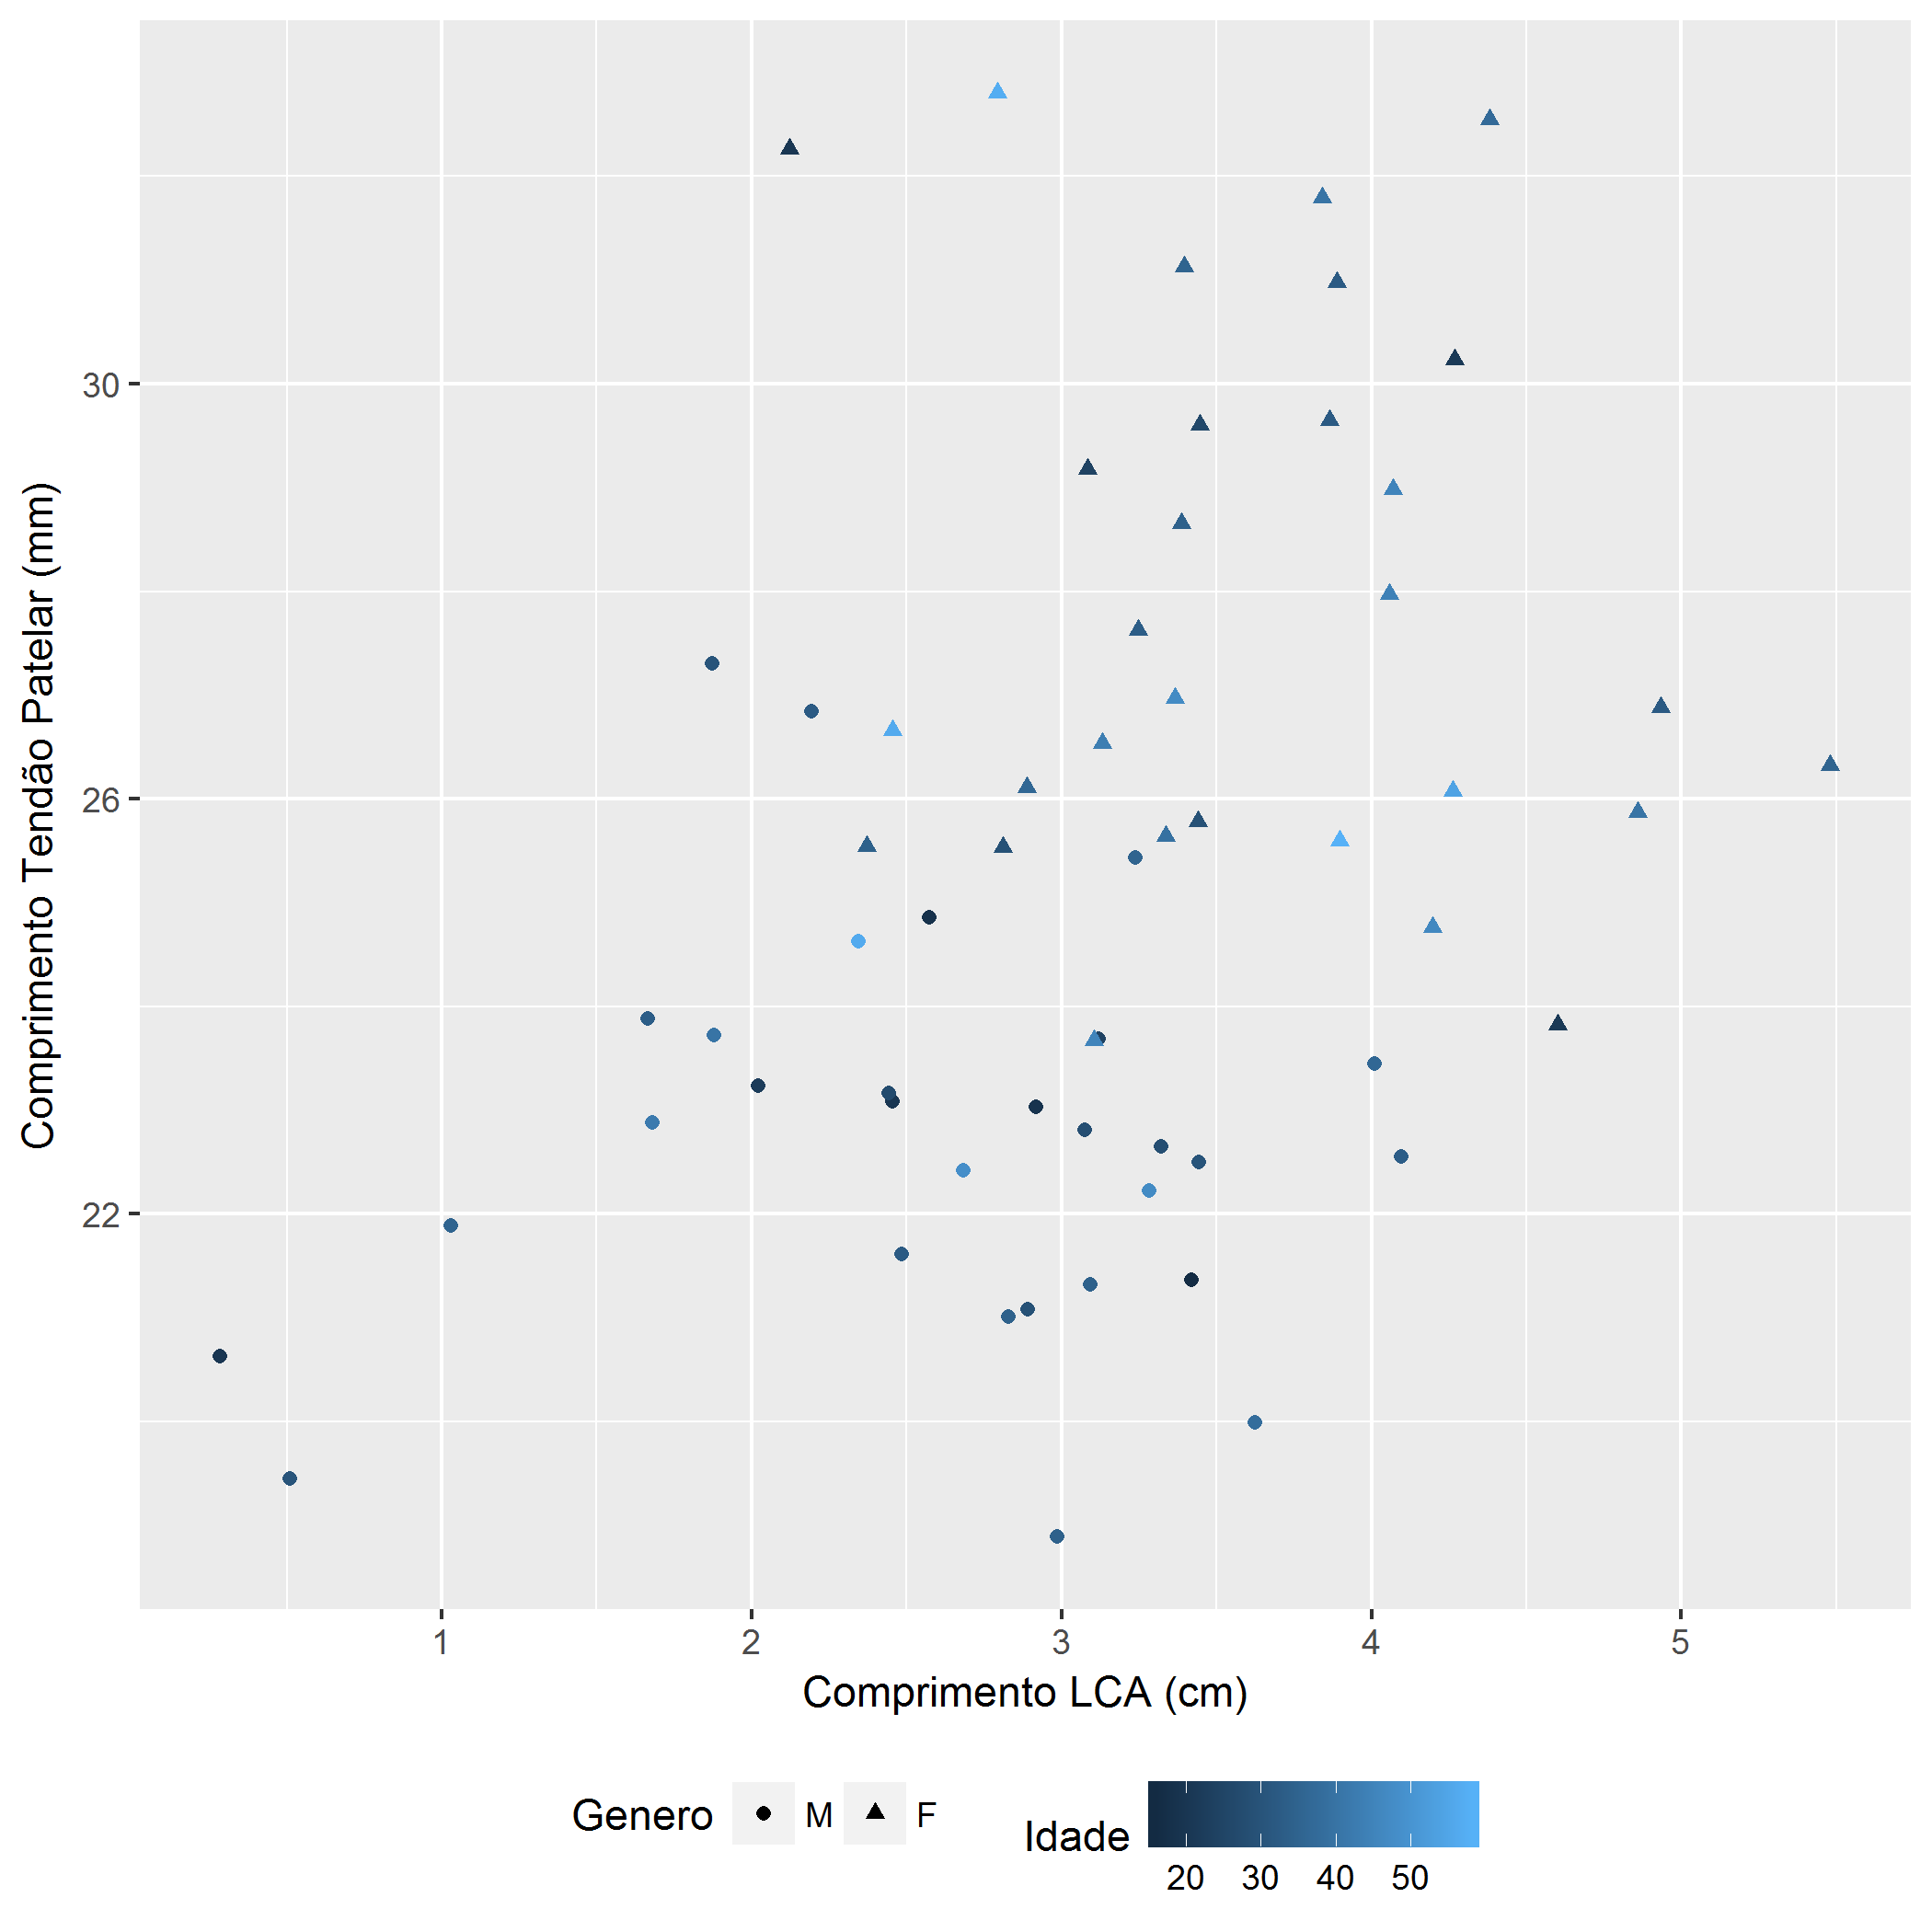
\includegraphics[height=.8\textheight]{EDA/EDA-corr3}
  \end{center}

  \vfill
  \tiny
  \hfill dados simulados com base no artigo
\end{frame}

\subsection{Resumo}

\begin{frame}{Resumo}
  \begin{enumerate}
    \scriptsize
  \item Não há escolha entre exploratória OU confirmatória -- ambas são importantes
    \bigskip
  \item É preciso pensar em ciência no sentido amplo, e não no paradigma linear
    \bigskip
  \item Para uma confirmação adequada, precisamos de um desenho cuidadosamente randomizado
    \bigskip
  \item Pensar em exploratória como uma atitude, não apenas como um conjunto de técnicas -- e usá-la antes da confirmatória
  \end{enumerate}

  \vfill
  \scriptsize
  \hfill Tukey, 1980
\end{frame}

\subsection{Referências}

\begin{frame}{Referências}
  \begin{itemize}
    \tiny
  \item Tukey (1980), We need both exploratory and confirmatory,

    {\tiny \url{http://www-ece.rice.edu/~fk1/classes/ELEC697/TukeyEDA.pdf}}

    (Acessado em 10/09/2015)
  \item NIST Handbook (1998), Exploratory Data Analysis, cap 1 --

    {\tiny \url{http://www.itl.nist.gov/div898/handbook/eda/section1/eda1.htm}}

    (Acessado em 10/09/2015)
  \item \href{https://doi.org/10.1002/0471264385.wei0202}
  {Behrens, Yu (2003), Exploratory Data Analysis, cap 2 -- Research Methods in Psychology}
  \end{itemize}
\end{frame}

\section{Aprofundamento}

\subsection{Aprofundamento}

\begin{frame}{Aprofundamento}
  \begin{block}{Leitura obrigatória}
    Não há.
  \end{block}
  \begin{block}{Leitura recomendada}
    \tiny
    Tukey (1980), We need both exploratory and confirmatory,

    {\tiny \url{http://www-ece.rice.edu/~fk1/classes/ELEC697/TukeyEDA.pdf}}

    (Acessado em 10/09/2015)
  \end{block}
\end{frame}

\end{document}
